\documentclass{ctexart}

\usepackage{newtxtext}
\usepackage{geometry}
\usepackage{tabularx}
\usepackage{graphicx}

\graphicspath{ {.} }
\geometry{a4paper, top=2.5cm, bottom=2.5cm, left=2cm, right=2cm}

\begin{document}

\begin{center}

\LARGE 2020 年福州市高一第二学期期末质量检测(不是)

\Huge \textsf{历 史 试 卷}

\bigskip

\normalsize(满分:100 分;完卷时间:90 分钟)

\medskip

\large \textsf{提示:答案请填写在答题卡指定的位置}

\end{center}

\textsf{一、选择题(以下各题都有一个正确答案,请将正确答案填在答题卡相应的位置。本大题共 26 题,每小题 2 分,共 52 分)}

1. 我国历史上第一个实行土地私有制的朝代是( )

\begin{tabularx}{\linewidth}{XXXX}

A. 夏朝 &
B. 商朝 &
C. 秦朝 &
D. 清朝

\end{tabularx}

2. “孟姜女哭长城”的故事,体现了秦朝实行( )

\begin{tabularx}{\linewidth}{XXXX}

A. 沉重的赋税制度 &
B. 沉重的徭役负担 \\
C. 严格的文化管制 &
D. 闭关锁国政策

\end{tabularx}

3. 下图的建筑修建于我国明代,体现了当时( )

\begin{center}

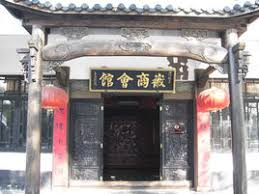
\includegraphics[scale=0.5]{3}

\end{center}

\begin{tabularx}{\linewidth}{XXXX}

A. 官方政府财力雄厚 &
B. 农民生活水平提高 \\
C. 产生区域性的大商帮 &
D. 出现资本主义萌芽

\end{tabularx}

4. “克拉克瓷”是古代一种用于出口的瓷器类别,因葡萄牙语中“巨型商船”被称作 Caraack 而得名。由此推断,克拉克瓷的产生时期约为( )

\begin{tabularx}{\linewidth}{XXXX}

A. 两汉时期 &
B. 隋唐时期 &
C. 宋元时期 &
D. 明清时期

\end{tabularx}

5. 韩非子在《五蠹》中写道:“夫明王治国之政,使其商工游食之民少而名卑,以寡趣本务而趋末作。今世近习之请行,则官爵可买;官爵可买,则商工不卑也矣。奸财货贾得用于市,则商人不少矣。聚敛倍农而致尊过耕战之士,则耿介之士寡而高价之民多矣。”,这体现了中国古代( )

\begin{tabularx}{\linewidth}{XXXX}

A. 社会崇尚正直的品质 &
B. 商人社会地位低下 \\
C. 官本位思想浓厚 &
D. 商业活动较为繁荣

\end{tabularx}

6. 19 世纪 50 年代初,一个在中国三个省份住了十年的英国人说道:“我还没有看见过一个靠劳作生活的中国人穿过一件用我们的布料做的衣服。”这说明( )

\begin{tabularx}{\linewidth}{XXXX}

A.外国商品没有进入中国 &
B.外国商品价格昂贵 \\
C.自然经济对外国商品的抵制 &
D.中国经济独立于世界

\end{tabularx}

7. 戊戌变法期间,保守派官员杨崇伊曾经就聘请日本前首相伊藤博文为顾问一事密奏慈禧太后:“风闻东洋故相伊藤博文,将专政柄。伊藤果用,则祖宗所传之天下,不啻拱手让人。”这体现了当时( )

\begin{tabularx}{\linewidth}{XXXX}

A.中外交流频繁 &
B.清朝学习外国政治制度 \\
C.部分官员思想较为保守 &
D.日本与中国较为友好

\end{tabularx}

\textsf{二、非选择题(本大题共 4 小题。第 27 题 12 分,第 28 小题 10 分,第 29 题 14 分,第 30 题 12 分,共 48 分)}

27.(12 分)阅读下列材料,回答问题。

\textsf{材料一}

\textit{铁发生影响的模式为人熟知。比以往工具生产效率更高的新式铁制工具使农业有可能从起初的黄河发源地向南扩展到森林茂密的长江流域(相当于从印度的印度河流域扩展到恒河流域)。铁制工具还促进了在大河流域地区兴修大批的排水工程、为远距离运输大批商品而进行的运河开挖以及在西北干旱地区进行的打井灌溉工程。}

\begin{flushright}

\texttt{——[美] L·S·斯塔夫里阿诺斯《全球通史》}

\end{flushright}

\textsf{材料二}

\textit{近代纺织企业,采用大机器生产,代表着社会生产力的新发展,引起了生产变革和社会变革。一方面,采用大机器生产的纺织企业,劳动生产率得到了很大提高。按照当时的生产水平,工人人均日产棉纱是手工纺纱的近 50 倍,人均机织布是手工织布的 6 倍多。劳动生产率的提高,反映了技术的进步和生产力的发展。另一方面,不论是官办、官督商办、官商合办,还是商办企业,都是以商品生产为目的,追求利润,因此都具有资本主义的性质,表明资本主义生产关系开始在中国出现。}

\begin{flushright}

\texttt{——汪圣云《论中国近代纺织工业的兴起及其历史作用》}

\end{flushright}

(1)据材料一并结合所学知识,简要概括我国古代农业技术的发展过程。(6 分)

(2)据材料一、二并结合所学,谈谈你对生产力的认识。(6 分)

\bigskip

27.(10 分)阅读下列材料,回答问题。

\textsf{材料一}

\textit{但是,列宁逝世后,斯大林在 1926 - 1928 年,虽然也讲过要建设工业,就应当从农业开始和工业是主导,农业是工业的基础,但在实践中却很快终止了新经济政策,并放弃了列宁的工业化道路。重新走上了类似于战时共产主义时期的工业化道路,即依靠农业来推动工业的发展,把农业当作高速度的工业化,特别是优先发展重工业积累资金和提供劳动力的主要源泉。致使苏联在经济发展的战略上出现了偏差。其主要表现是,重工业的发展不是建立在为农业、轻工业服务的基础上,而是建立在重工业自我服务、自我循环的基础上。由于片面发展重工业,农业生产长期上不去,经常出现农业歉收和粮食危机现象。结果,重工业虽然发展了,但是农业和轻工业却陷于停滞状态,从而使得国民经济各部门的比例关系严重失调,结果势必影响包括工业在内的整个国民经济的健康发展,特别是造成农业的长期落后,农业生产一直徘徊在沙俄时代水平。1953 年同 1913 年相比,苏联工业总产值增长了 18.36 倍,而农业总产值仅增长了 46\%。}

\begin{flushright}

\texttt{——詹真荣《前苏联共产党处理农业和农民问题的教训》}

\end{flushright}

\textsf{材料二}

\textit{中华民国政府迁台后,时任中华民国总统蒋中正将台湾视为以武力反攻大陆的基地,奉行军事优先和稳定农业的经济政策。自 1960 年代起,台湾轻工业发展快速,重工业则居于次要地位。中央政府为了增加出口换取外汇,还设立加工出口区来增加外贸收入。}

\textit{到了蒋经国时代,为摆脱石油危机,中央政府致力推动十大建设,为台湾石化业与重工业打下良好的基础,此时恰逢越南战争,美国向台湾订购大量物资,这些因素都促使台湾经济快速起飞。由于经济发展成功,台湾遂晋身亚洲四小龙行列,亦达到新兴工业化国家水平。之后中央政府注意到重工业在经济中的地位,实行积极的产业政策,在高雄建设大炼钢厂、大造船厂、大炼油厂等大型重工业基地,亦有外资,中央政府,加上华侨返台的科技资本,因而设立电子科技公司,如台积电、联华电子等也取得成功。}

\begin{flushright}

\texttt{——维基百科《台湾奇迹》}

\end{flushright}

(1)据材料一并结合所学知识,指出苏联工业化过程中的不足。(4 分)

(2)据材料一、二并结合所学,谈谈应该如何较好地实行国家的工业化。(6 分)

\end{document}
